\chapter{Background \& Related Work}

\section{Parallel vs. Distributed Computing}
Before detailing the most prominent continuing projects in this space, it is important to draw a distinction between parallel and distributed computing. In order to do that, clear definitions for parallel and distributed computing must be provided. While this thesis project will primarily be geared toward distributed applications running in high-performance computing (HPC) settings, it will also attempt to exploit parallelism, so understanding both is essential for a holistic view of the space in which the proposed project will exist. Definitions included below are a mixture of universal standards used in literature and what will be considered distributed/parallel computing for the purposes of this project.

\begin{figure}[h]
\centering
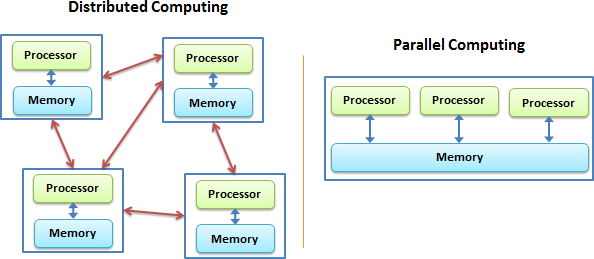
\includegraphics[width=0.65\textwidth]{Figures/parallel_vs_distributed.png}
\caption{Visualization of the difference from \cite{dist_java}. These red lines represent internal connections within a cluster. This is obviously a simplifcation, as all of these lines would likely be connected to a switch or some other communication mechanism.}
\label{fig:dist_v_parallel}
\end{figure}

\paragraph{Parallel Computing}
There are two main modes of parallelism in parallel computing: instruction-level parallelism and thread-level parallelism. 

Instruction-level parallelism refers to design techniques at the processor/compiler level that speed the execution of sequential programs by allowing individual machine instructions, e.g. additions, floating point multiplications, memory stores/loads, to execute in parallel \cite{ilp_history}. This is typically done using different components of a processor to perform different parts of a given instruction at the same time. Modern processors typically have, at the very least, several floating point units and several integer units, which can handle different parts of the same instruction. Processors that are capable of intstruction-level parallelism are called \textbf{superscalar} processors.

The main distinction between instruction-level parallelism and thread-level parallelism is that instruction-level parallelism occurs at the processor level whereas thread-level parallelism exploits concurrency among multiple processors within the same computer \cite{hpc_openstax}. When these threads share memory in addition to processing resources, the computer on which the threads are running is said to have a \textbf{shared memory architecture}. The thread in thread-level parallelism refers to a thread of execution in which some part of a program runs its code. Threads are different from processes in that threads share the same memory space and are all added to the same existing process. These attributes give threads a distinct advantage over processes when one is working with multiple processors, as an arbitrary number of threads can work on the same shared data structure, either through synchronization or through splitting the structure up into discrete parts \cite{hpc_openstax}. 


\paragraph{Distributed Computing}
The distinction between parallel computing and distributed computing is much like the distinction between instruction-level parallelism and thread-level parallelism.  Instruction-level parallelism occurs within one processor, while thread-level parallelism occurs in a system with multiple processors. Similarly, parallel computing occurs within one computer, while distributed computing occurs across multiple computers. Naturally, new and unique problems arise when a project migrates from a single system of computers to a cluster consisting of multiple computers that are just as challenging as the problems that arise when making sequential code parallel. Common problems include, but are not limited to heterogeneity in networks, hardware, programming languages, or implementation of standard constructs, openness of components within a distributed system, scalability, fault tolerance, concurrency of different resources across different machines, and unique quality of service (QoS) issues relating to availability, reliability, and performance that do not affect applications running on a single computer \cite{dist_systems_concepts}. Distributed computing can refer to anything from blockchain networks, which distribute verification of information and transactions across many different systems, to web services architectures, in which a web application is broken into modular, discrete components which then run on different computers and communicate across the network, to cloud computing, in which innumerable virtual private servers are spun off and destroyed in tandem across many machines in a massive data center. This project will mainly focus on HPC settings in which memory-intensive scientific applications are run, but hopefully the deliverable will be able to be extended to cloud computing environments, and perhaps even to desktop computer environments if the memory management methods are applicable at this smaller scale. For the purposes of this project, computers with a discrete GPU or other processing component will not be considered distributed computing since many of the aforementioned challenges are less relevant when communicating between components within the same machine - offloading operations to a GPU is analogous to offloading to another CPU core or offloading cache contents to RAM.  
\newpage
\section{Problem Domain: P-Complete Problems}
In complexity theory, the $NP$ and $P$ classes are well known: $P$ represents all decision problems which can be solved in polynomial time by a deterministic Turing machine, whereas $NP$, a superclass of $P$  represents all problems which are not known to have polynomial time solutions. There is also another subclass of $NP$ disjoint from $P$  called $NP$-complete problems, into which all problems in $NP$ can be reduced. While the daunting question of whether $P = NP$ remains open, we generally consider NP-complete probables \textit{intractable}, meaning that they are probably not in $P$. Less discussed is the similar class structure which exists within the $P$ subclass. There exist two well known subclasses of $P$, $NC$ and $L$, which have a standing comparable to $P$'s within $NP$ \cite{Sipser_2006}. $NC$ contains all problems which are parallelizable in poly-logarithmic time using a logarithmic number of processors, while $L$ contains problems which are decidable in logarithmic space \cite{Greenlaw_Hoover_Ruzzo_1995}. Additionally, there exists another subclass of $P$ disjoint from $NC \cup L$ called the $P$-complete problems. Like with $NP$ and $P$, it is not known whether $NC$, $L$, or even $NC \cup L$ is equal to $P$, but the $P$-complete problems can be considered as those problems which are probably not easily parallelized and/or deciable in logarithmic space. 

One essential example of a $P$-complete problem is the subgroup containment problem, which asks whether two generated subgroups are the same. Many linear programming problems, graph theory problems, and number theory problems fall into the $P$-complete class. An excellent compendium of known $P$-complete problems, along with some proofs and explanations, can be found in \cite{Alvarez_Greenlaw_2000}. In general, these are interesting, generic problems applicable to many different disciplines. However, the study of high performance computing is typically focused on achieving maximum performance from problems in $NC \cup L$ while avoiding tailoring frameworks to the specialized needs of $P$-complete problems. PC2L aims to provide a framework which can support these types of inherently sequential and/or memory intensive problems. 

\section{Locality of Reference}
In Central Processing Unit (CPU) design, as well as low-level kernel programming, engineers and computer scientists must consider the pattern in which processors are likely to access data so that said data can be provided as fast as possible, preferably without the processor noticing. For example, if a processor is going to access and increment a 64 bit integer $2^{60}$ times, it would be preferable to have this integer in the CPU's cache, a small, incredibly fast section of memory, instead of the hard disk, which is a larger, and comparatively slow part of computer memory. The pattern in which a processor accesses data is termed locality of reference (LOR).

In the case of PC2L, we will be attempting to predict the pattern in which code in the operating system's userland which implements our library accesses memory instead of how the processor accesses memory, but we will still be utilizing LOR. There are several different subtypes of LOR which will have to be accounted for \cite{Stallings_2010}. Spatial LOR is when one data access within an interval predicts another data access within the same interval. Temporal LOR is when accessing one address in memory means that the same address will likely be accessed once more after a given time interval. Branch LOR is when memory in certain regions is most likely to be accessed because of the rigid structure of the userland program in our case, or the assembly instructions for the processor in the lower level case. These flavors of LOR can be combined to produced other distinct LORs. For example, perhaps a program's next memory access can be predicted by a combination of the interval it last accessed (spatial) and the data it most recently accessed (temporal). 

\section{Cache Replacement Policies}
As mentioned in the previous section, a CPU's cache space is a low storage, low latency, high bandwidth memory module. A CPU's cache is built into the silicon of the CPU itself in order to achieve the minimum possible distance from where processing occurs. Similarly, companies like Facebook, Imgur, and Twitter cache their content on closer computers and/or user machines in order to achieve faster applications and minimize expensive requests. While understanding the power of caches is an essential part of the software engineering process, we will mostly be focusing on the knowledge that we can take away from the immense pool of research pertaining to general caches, and how said knowledge applies to our use case within a distributed computing cluster. One of the main pieces of lower level knowledge that may apply to the way PC2L manages the resources of userland programs is cache replacement strategy.

Cache replacement strategy refers to the decision process that leads to a chunk of memory being evicted from the cache. Typically this is predicated on the idea that caches have limited storage, and allowing information that will not be accessed again to hold space in the cache will drain performance. There are several heuristics for answering the question of which memory chunks should be evicted from the cache, and each one lends itself to different situations. One of the main strategies utilized in any kind of cache is least recently used (LRU) caching, which will evict the object with the oldest access date. Another common strategy is least frequently recently used, which is an implementation of LRU caching that prvileges popular entries, combining time and frequency of use to decide which entry should be evicted next. There is also time aware LRU caching, which adds a TTL component to entries in the cache, removing entries regardless of frequency after they have been in the cache for a certain period of time. 

As mentioned before, each of these strategies lends itself better to different use cases. For example, previous research has found that a most recently used (MRU) replacement algorithm beat out all other replacement strategies when a looping sequential locality of reference was being used \cite{Chou_DeWitt_1986}. One of the main tasks in developing PC2L will be identifying the LOR for a given userland application and attempting to choose our cache replacement policy based on this information. 
\section{First-Class Distributed Computing in C++} \label{first_class_dist_cpp}
While the most powerful computers in research in industry continue to expand their processor and GPU counts,
distributed computing is not yet included as a first class component of the C++ Standard Templating Library (STL) \cite{towards_dist_cpp}. This forces many developers of high-performance scientific applications to "reinvent the wheel" for each individual project.  Common parallel computing constructs, like threads, mutexes, and other locks, went through a similar process in C++. Exploring the history of other attempts to standardize distributed data structures, as well as analogous constructs, is essential to understand the full picture of distributed computing in C++. First, we will detail the existing constructs for parallel and distributed computing and the history of their rise from community-driven tools to first class members of the STL. Next, we will explore recent attempts to add distributed computing paradigms into the C++ STL. 


\paragraph{Existing Constructs}
Despite the lack of distributed constructs in C++, there are many objects used in heterogeneous/parallel computing that serve as important references for any distributed data structures/algorithms. Most important among the aforementioned constructs are \texttt{std::async}, \texttt{std::future}, \texttt{std::atomic}, \texttt{std::mutex}, \texttt{std::unique\_lock}, and \texttt{std::thread}, which are detailed in proposals N1682, N1815, N1875, N1883, N1907, N2043, N2090, N2094,  N2096, N2139, N2178, N2184, N2885, and N2889, among others  \cite{n1682} \cite{n1815} \cite{n1875} \cite{n1883} \cite{n1907} \cite{n2043} \cite{n2096} \cite{n2139} \cite{n2178} \cite{n2184} \cite{n2285} \cite{n2889}. A great summary and amalgam of all these proposals can be found in N2320 \cite{n2320}. Figure \ref{fig:cpp_firstclass} provides a summary of the relationships between these constructs.

To briefly summarize this history, before the ISO C++ STL  implemented threading or any concurrency at all, Boost, a popular library that extends the STL, had its own version of threads, locks, and other essentials for concurrency. After the entire Boost community and development team had troubleshooted, iterated, and improved these features in boost, they had an outstanding product with fairly widespread industry adoption. Since the C++ working groups (WGs) have less flexibility and agility in the implementation of a new feature, they did not get around to discussing threading in C++ until after Boost was a full-formed library. As a result, the multi-threading library in the STL is opaquely influenced by Boost. C++ threads, just like boost threads, can be waited on, cooperatively cancelled, quereied, joined with other threads, detached, and otherwise managed. \texttt{std::mutex} in C++ is the mechanism by which threads are locked and synchronized. This ISO adoption of Boost standards is encouraging for any developer who wants to spin up a useful open-source library for use in the community, as it demonstrates that libraries with enough widespread community support can eventually become first-class members of the C++ STL. 

The idea of a standardized object for resolving an asynchronous subroutine call arose as a result of the fact that though there were many different multi-threading APIs proposed for the C++ standard, each of these libraries made simply calling another subroutine in parallel a difficult task with high code complexity. The intended domain for \texttt{std::async} was extracted concurrency in existing programs. There existed, and still exist, a number of applications that are purely sequential, having been written before multi-threading was widely possible, and inserting a function call in a couple of places is usually a more realistic goal than rewriting entire applications with concurrency in mind. N2889 gives the example of quicksort: \texttt{std::async} would be appropriate for recursive calls to quicksort, but not to the iteration in a partition, as it was not intended to compete with existing loop-parallelism solutions. \texttt{std::future} is the type returned by a call to \texttt{std::async}, and was proposed for this purpose instead of \texttt{std::unique\_future} to avoid unnecessary overhead. \texttt{std::future} can be thought of as a more primitive thread, in that it doesn't not provide any method for synchronization. 

Threads are relevant for the purposes of this project since thread-level parallelism will be necessary to maintain any concurrent data structure at a node level. Additionally, passing, cancelling, or locking threads from node to node may be essential depending on the implementation of our concurrent data structures, which seems to indicate that either using some implementation of thread pools or creating our own may be necessary. \texttt{std::future} is relevant for work that does not require synchronization, and a distributed implementation of future could be interesting, as it could potentially offer easy speed improvements to poorly written HPC applications. 


\begin{figure}[h]
\centering
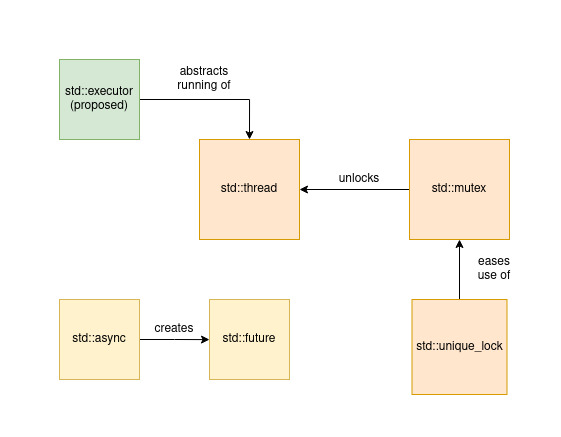
\includegraphics[width=0.65\textwidth]{Figures/cpp_firstclass.jpg}
\caption{Relationships between existing and proposed C++ constructs}
\label{fig:cpp_firstclass}
\end{figure}

\paragraph{Recent attempts}
Among the most compelling recent attempts to include distributed constructs in the STL is the proposal P0443 \cite{p0443}. Driven by the increasing diversity and heterogeneity of hardware within almost every system from the newest smart phone to HPC clusters, this proposal suggests the creation of a work execution interface, \texttt{std::executor}. Additionally, the proposal calls for representations of work/the relationships between work, \texttt{std::sender} and \texttt{std::receiver}. The executor interface could be used to represent anything from a thread pool to SIMD units to GPU runtimes to the current thread. Programmers could author executors by defining their own execution functions for each of these very different environments, and the executor interface is likely robust enough to provide support for any other execution environments that might arise in the future. Senders and receivers can represent almost any relationships between work in a flow diagram, allowing for the development of more generic code that acts on an asynchronous dependency graph and can be moved seamlessly in-and-out of systems with significant hardware differences. 

An interesting addition to P0443 is the application of affinity to executors as described in \cite{towards_dist_cpp}. In this context, affinity refers to memory access performance between running code and the data accessed by said code. In this context, a resource has higher affinity with a section of memory if access of that section comes with lower latency and/or higher bandwith \cite{towards_dist_cpp}. The authors suggest tailoring the executors detailed in P0443 to allow for application developers to preemptively place data/threads in the right place according to affinity, making it so that applications do not have to rely on the operating system to allocate each particular part of memory to the highest affinity segment, perhaps speeding memory accecss and/or achieving more bandwith. 

While both of these ideas would likely mesh excellently with this project, unfortunately neither have made it into any recent C++ standards. The current C++ machine model is still strictly CPU focused \cite{towards_dist_cpp}, and thus does not account for GPUs or other heterogeneous components, much less other computers. However, the approach of allocating memory based on affinity within an application instead of relying on the operating system is incredibly relevant for this project, as we will likely have to design our solution to optimize affinity on both a node level and a cluster level, where affinity with each big memory node must be accounted for.  

\section{Memory in Distributed Applications} \label{memory_distrib}
Since the beginning of the information era, there has been rapid development of better CPUs with increased cores and faster clock times in conjunction with an increase in demand of data accesses in many applications \cite{sharing_cpu_memory}. Since the affordability and speed of RAM has not followed that of CPUs, this means that the memory resources in a distributed system are now much more expensive relative to CPU cycles. As a result of this, any interventions that improve the efficiency of accessing and sharing memory, whether at an operating system level or user level, could greatly improve the profitability and efficiency of existing distributed applications. Literature presents several existing improvements to memory usage in distributed applications like \cite{virtual_memory_tlb} \cite{sharing_cpu_memory}.

\begin{figure}[h]
	\centering
	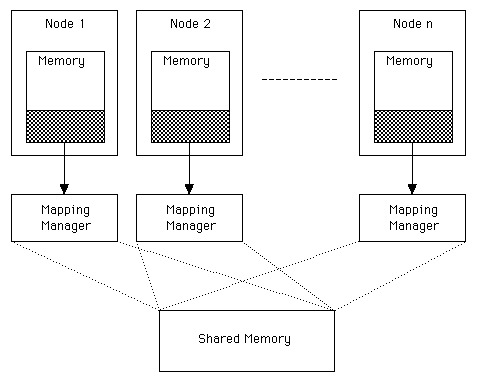
\includegraphics[width=0.65\textwidth]{Figures/dsm.jpg}
	\label{fig:dsm}
	\caption{Distributed Shared Memory \cite{vt_cs}}
\end{figure}
Some of the main challenges in architecture of a shared memory system include coherence enforcement, coherence protocol, processor system interfacing, and interconnection network utilization \cite{challenge_dist_mem}. In this context, coherence refers to determining which instance of a given piece of memory can be considered accurate. For example, a distributed system may cache 4 redundant copies of the same block of memory on 4 separate nodes to speed reading this block. When one node updates this block of data, all 4 must be notified, and the value must be changed in all of their local caches. Processor system interfacing refers to interactions a distributed application might have with distinct processors on distinct machines. For example, one processor may be little-endian whereas another is big endian. For the purposes of this project, this subtle, yet important, issue will initially be ignored in favor of shipping a viable product for Miami University's cluster, then addressed after a sufficiently featured prototype is working. Extra attention will be paid to using/implementing the most efficient coherence protocol while still achieving acceptable coherence enforcement.  

In light of all the potential pitfalls surrounding distributed memory and the abundance of programs that rely more on intensive data access than repeated operations, designing a framework that is intended specifically to work with these kind of specialized applications seems to be a desirable goal. 

\section{Application Binary Interfaces}
\begin{figure}[h]
	\centering
	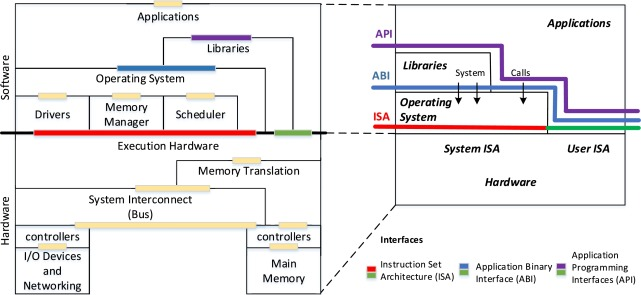
\includegraphics[width=0.5\textwidth]{Figures/abi.jpg}
	\label{fig:abi}
	\caption{ Hardware/Software diagram of a typical system. ABI is in blue. \cite{virtualization}}
\end{figure}
Since the scope of this project is fairly low level, some exploration of how the operating system handles the transfer of data from program to program is necessary, as similar methods will be used when transferring data from machine to machine. Just as an Application Programming Interface (API) defines how users of an application should use exposed methods in a human-readable format, the application Binary Interface defines how programs should use exposed machine methods. AMD's System V ABI for x86 and x64 systems \cite{amd_x86_64} is one example of how an ABI might look in the real world.




While dealing with ABIs is typically the job of the compiler or the operating system, there are obvious benefits for framework developers who know the ins-and-outs of industry ABIs. For example, if the runtime system for the framework that is developed for this project ends up using caching, and C++ objects have to be transferred around from machine to machine, they will likely have to be transferred in either binary or some condensed form of binary, and we must know how to translate this back into an object that is received into an understandable format for the recieving machine. Knowing at least some basic calls to the ABI could be an essential part of caching objects at a node level, and will likely play a role in our coherence protocol. 

Additionally, dealing directly with the applcation binary interface could prove to be the most performant solution for our program. If we intended to cache data at the node level, we could simply store it in binary, or some compressed binary, format, moving it around from node to node in the cluster and making calls to the ABI to get it into the instance of our application that is running on a particular node. 
\section{Related Work}
\begin{table}[]
\centering
\resizebox{\textwidth}{!}{%
\begin{tabular}{|l|l|l|l|l|l|l|l|}
\hline
Project   & Paradigm & Architecture & Nested & Adaptive & Data Dist. & Scheduling            & Continued development \\ \hline
STAPL     & S/MPMD   & Shared/Dist  & Yes    & Yes      & Auto/User  & Customizable          & Yes                   \\ \hline
PSTL      & SPMD     & Shared/Dist  & No     & No       & Auto       & Tulip RTS             & No                    \\ \hline
Charm++   & MPMD     & Shared/Dist  & No     & No       & User       & prioritized execution & Yes                   \\ \hline
CILK      & S/MPMD   & Shared/Dist  & Yes    & No       & User       & work stealing         & No                    \\ \hline
NESL      & S/MPMD   & Shared/Dist  & Yes    & No       & User       & work and depth model  & No                    \\ \hline
POOMA     & SPMD     & Shared/Dist  & Yes    & No       & User       & pthread scheduling    & No                    \\ \hline
SPLIT-C   & SPMD     & Shared/Dist  & Yes    & No       & User       & user                  & No                    \\ \hline
X10       & S/MPMD   & Shared/Dist  & No     & No       & Auto       & -                     & Yes                   \\ \hline
Chapel    & S/MPMD   & Shared/Dist  & Yes    & No       & Auto       & -                     & Yes                   \\ \hline
Titanium  & S/MPMD   & Shared/Dist  & No     & No       & Auto       & -                     & No                    \\ \hline
Intel TBB & SPMD     & Shared       & Yes    & Yes      & Auto       & work stealing         & Yes                   \\ \hline
\end{tabular}
}
\label{Tbl:comp_tbl}
\caption{Comparison between different distributed solutions in or resembling C++ \cite{STAPL_2010}.}. 
\end{table}
\normalsize
There exist a number of comparable libraries that have attempted to standardize commonly used distributed/parallel structures, or otherwise create a standard library for distributed computing in C++. Out of all of the libraries initially created to address distributed computing in C++, however, few are still in continued development in 2021. The comparison table lists libraries for distributed and parallel computing in C++. Some of these libraries have created their own language (Chapel/Cilk) based heavily on C/C++ specifically to support their run-time system (RTS). Others, like Charm++, have created their own interoperable message passing interface for communication between processors and nodes.  One additional significant difference not readily visible on the table is that none of these libraries attempt to solve any of the difficulties inherent in memory-bound distributed applications. Additionally, there are numerous solutions dedicated to speeding distributed computing with large in-memory components, including Spark, Memcached, and Globally Addressable Memory (GAM). Brief overviews of the architecture and contributions of each of these solutions are provided below.   

\subsection{STAPL}
\begin{figure}[h]
\centering
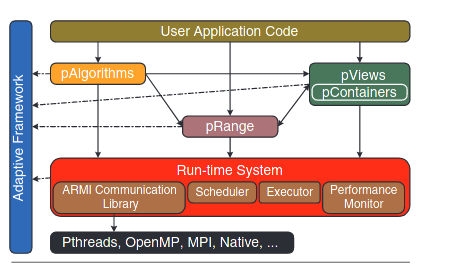
\includegraphics[width=0.5\textwidth]{Figures/stapl_overview.png}
\caption{STAPL Architecture \cite{stapl_parallel_container}}
\label{fig:stapl_arch}
\end{figure}
\paragraph{Description} 
The Standard Template Adaptive Parallel Library (STAPL) was developed by researchers at Texas A\&M University in the late 1990s, far before the C++11 standard provided a set of standardized tools for concurrency. The library was originally created as a super-set of C++'s STL, with the intent to possibly replace the STL on small to medium multiprocessing systems \cite{STAPL}. STAPL is capable of running both single program multiple data (SPMD) and multiple program multiple data applications, and its scheduling algorithm is customizable. STAPL, like the C++ STL, is a generic library, offering data structures and algorithms that can be exploited by a large number of heterogeneous applications. \cite{STAPL}. STAPL implements each distributed data structure as a thread-safe, concurrent object called a pContainer \cite{stapl_parallel_container}. 

STAPL pContainers consist of a finite collection of typed elements, storage space, and an interface of methods/procedures that can be applied to the pContainer. \cite{stapl_parallel_container} Each pContainer is globally addressable, meaning it provides shared memory address space, and can be composed with other containers to create new structures \cite{stapl_parallel_container}. Distributed data structures implemented by STAPL include an array, a vector, a list, a matrix, a graph, a map, and a set \cite{stapl_parray} \cite{stapl_graph}. The library also includes common algorithms for these data structures like those one would find in the C++ STL. 

STAPL facilitates communication between data structures and algorithms by having algorithms communicate with pViews through pRanges in the same way that algorithms in the C++ STL communicate with iterators \cite{stapl_parallel_container}. STAPL represents most algorithms using compositions of algorithmic skeletons, which include many common interaction patterns in parallel programs; for example, map, reduce, zip, and gather \cite{stapl_skeleton_framework}. Providing standard, efficient implementations of these skeletons allows users of the framework to focus on the business logic of their program instead of generic patterns. The code sample below includes an example usage of a few of these algorithmic skeletons. 

Like many of the other C++ libraries designed with distributed/parallel computing in mind, STAPL provides its own custom runtime system detailed in \cite{stapl_rts}. One of the main ideas in STAPL's runtime system is that of a paragraph, which is essentially a directed task graph in which each work items are represented by vertices and dependencies are represented by edges. The runtime system provides executors and schedulers for the tasks detailed in pRanges \cite{STAPL_2010}.
\paragraph{Contributions} 
\begin{itemize}
	\item
		\textbf{Adaptive Remote Method Invocation (ARMI)}. STAPL provides primitives for registering parallel objects and using Remote Method Invocation on them from any cluster machine. This allows for the asynchronous transfer of data and work throughout the distributed system.  ARMI utilizes the future and promise constructs detailed in \ref{first_class_dist_cpp}. 
	\item
		\textbf{Generic Distributed Containers (pContainers)}. The STAPL parallel container framework provides a good way of abstracting away the implementation details of a given container on a distributed system, giving users a generic interface that works with any parallel container regardless of the type of system or network on which it is exists. In addition to a good interface, STAPL provides its own implementations of containers that stack up well against other industry-standard implementations in scalability and performance trials. \cite{stapl_parallel_container}.	
	\item
		\textbf{Shared Memory Abstraction}. For users who are not working on lower-level applications, STAPL provides an abstraction of the global memory. For more advanced users, STAPL exposes a partitioned global addres space (PGAS) architecture. 

		\textbf{Big Data Graphs}. This is a particularly interesting contribution for this project. STAPL's graph library \cite{stapl_graph} provides a novel approach to out-of-core processing for big data graphs in memory-constricted systems, allowing algorithms implemented in this library to efficiently process graphs that do not fit entirely in RAM. STAPL's parallel graphs use a novel approach that combines RAM and hard disks/SSDs, and works exceedingly well on large distributed memory networks. The approach is comparable to paging, loading subgraphs of a larger graph into available RAM until the whole graph is processed. 
\end{itemize}

\paragraph{Code sample}
This code solves the first project euler problem, which asks for the sum of all numbers below $n$ that are multiples of 3 or 5. \cite{euler_1}. The code was retrieved from the examples section of STAPL's Gitlab repository. 
\scriptsize
\begin{lstlisting}[language=C++, caption=STAPL code sample for Project Euler number 1. Headers and doxygen comments removed for brevity, captionpos=b]

typedef unsigned long long ulong_type;

struct three_five_divisor
{
  template<typename T>
  bool operator()(T i)
  {
    return !((i % 3) == 0 || (i % 5) == 0);
  }
};


stapl::exit_code stapl_main(int, char** argv)
{
  ulong_type num = boost::lexical_cast<ulong_type> (argv[1]);

  // Creates array container of unsigned integers that will be used for storage.
  stapl::array<ulong_type> b(num);

  // Creates view over container.
  stapl::array_view<stapl::array<ulong_type>> vw(b);

  // Fills the container with values from 1 to n.
  stapl::iota(vw, 1);

  // For numbers in the container that return true to the three_five_divisor
  //   functor, they are set to 0.
  stapl::replace_if(vw, three_five_divisor(), 0);

  // Adds the total of all elements in container.
  ulong_type total = stapl::accumulate(vw, (ulong_type)0);

  // Prints the total sum.
  stapl::do_once ([&] {
    std::cout << "The total is: " << total << std::endl;
  });

  return EXIT_SUCCESS;
} \end{lstlisting}
\normalsize
\subsection{Charm++}
\begin{figure}[h]
	\centering
	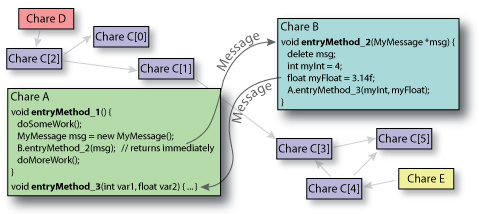
\includegraphics[width=0.5\textwidth]{Figures/charm_arch.jpg}
	\caption{Charm++ Architecture \cite{charm_tutorial}}
	\label{fig:charm_arch}
\end{figure}
\paragraph{Description} \label{charm_desc}
Charm++ is a parallel programming framework designed to ease the development, execution, migration, and decomposition of parallel applications \cite{parallel_programming_w_charm}. First developed in the early 1990s, Charm++ may have been one of the earliest frameworks to attempt to address distributed computing issues with object-oriented solutions. When Charm++ was first brainstormed, both object orientation and concurrency were still relatively novel. Charm++ was especially innovative among early object-oriented concurrent frameworks in that it allowed for abstractions of modes of information sharing and communication, provided support for load balancing and prioritization, and put forth a new "chare" object used for programming common data parallel applications \cite{charm_93}. 

A chare is essentially a parallel process which can spin up more chares and send messages to other chares. In this sense, the Charm++ framework is only a step above MPI in that it provides additional features on top of the bare-bones parallel process management system. Some of these features include data abstractions for information sharing, such as read-only data, accumulators, monotonic/atomic variables, and distributed tables \cite{charm_93}. 

Additionally, over a decade before the STL accepted future and async as members, Charm++ included its own implementation of future, which is basically follows the same idea as the STL implementation discussed in \ref{first_class_dist_cpp} in that the calling process blocks until the value in the future is computed. 

Unlike STAPL and some other framework's in this domain, Charm++'s runtime system is message driven, and every Charm program can broadly be defined, much like MPI, as an initialization and a message-driven loop \cite{charm_rts}. In the initialization, the user defines a main chare and branch chare, initializes a memory manager, crafts queue management devices, and deals with load balancing, among other things. In the mesage driven loop, termed a "pick and process loop", the runtime system essentially acts as a work pool manager, comparable to an executor in a thread pool except with messages instead of threads. Users choose how messages are picked, defining distinct message priorities as necessary for different applications.  
\paragraph{Contributions}
	\begin{itemize}
		\item \textbf{Message driven runtime system}. Whereas many frameworks abstract away the concept of messaging such that the user does not have to deal with it, Charm++ is entirely based around messaging. All objects are built around sending and processing messages. While this can induce a learning curve for Charm++, it also makes programs written in Charm++ more readable for advanced users.  
		\item \textbf{Latency tolerance through futures}. As mentioned in \ref{charm_desc}, Charm utilizes largely the same future construct that is used in the C++ STL. This makes transitioning trivially data parallel applications to Charm much easier, as the futures can simply be swapped out.   
		
	\end{itemize}

\paragraph{Code sample}
This code prints hello world on a single processor using a single chare in Charm++. It is difficult to show any other simple programs, as Charm++ programs often exist across a header file, source file, interface file, and involve a nontrivial degree of code complexity.
\scriptsize
\begin{lstlisting}[language=C, caption=Hello World in Charm++ from \cite{charm_tutorial}, captionpos=b]
// File: main.h
#ifndef __MAIN_H__
#define __MAIN_H__

class Main : public CBase_Main { (1)

 public:
  Main(CkArgMsg* msg); (2)
  Main(CkMigrateMessage* msg); (3)

};

#endif //__MAIN_H__


// File: main.c

#include "main.decl.h" (6)
#include "main.h"

// Entry point of Charm++ application
Main::Main(CkArgMsg* msg) {

  // Print a message for the user
  CkPrintf("Hello World!\n"); (4)

  // Exit the application (5)
  CkExit();
}

// Constructor needed for chare object migration (ignore
// for now) NOTE: This constructor does not need to
// appear in the ".ci" file
Main::Main(CkMigrateMessage* msg) { }

#include "main.def.h" (6)
	
// File: main.ci (interface)
 mainmodule main { (7)

  mainchare Main { (8)
    entry Main(CkArgMsg* msg); (9)
  };

};

\end{lstlisting}%

\normalsize

\subsection{X10}
    \begin{figure}[ht]
		\centering
		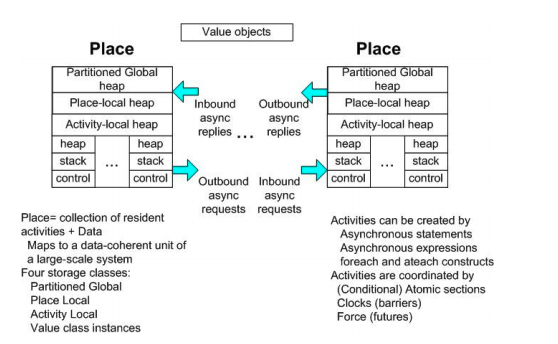
\includegraphics[width=0.50\textwidth]{Figures/x10_arch.png}
		\caption{X10 Architecture \cite{X10_2005}}
        \label{fig:x10_arch}
    \end{figure}
	\paragraph{Description} \label{X10_desc}
X10 was developed in 2004 as part of IBM's Productive Easy-to-use Reliable Computer Systems (PERCS) project, partially because its authors felt that concurrent interactions in languages like Java were too technically complicated to be grasped by the majority of practicing programmers \cite{X10}. While the two frameworks mentioned so far attempted to add acccess to distributed memory to C++ as part of frameworks, X10 is an attempt to create an entirely new language dedicated to distributed and parallel computing. X10 is not alone in this category: there are a multitude of programming languages or language spin-offs created solely for this purpose, including, but not limited to High Performance Fortran, ZPL, Titanium, Co-Array Fortran, SPLIT-C, Unified Parallel C, and CILK. X10 deserves more of a spotlight than these languages in the context of this project because it is heavily based on C++, the target language for our proposed framework, and because, like the other frameworks outlined here, it had its own approach to sharing distributed memory through a PGAS. X10's language features are largely irrelevant for the purposes of this proposal; it suffices to say that X10 is a static, strong, and safely typed compiled object-oriented language that shares many of the features of C++. 

An essential concept in X10 is that of a \textit{place}, which is a collection of light-weight threads, termed \textit{activities}, and data. Since the language was designed with high-performance scientific computing in mind, these places were intended to correspond with nodes in a cluster, but could also correspond with one coprocessor in a commercial machine. X10 allocates storage on the activity and place level, with a unified PGAS for remote activities and additional storage allocate for \textit{values}, which are immutable, stateless classes comparable to immutable plain old data (POD) objects in other languages. 

X10 replaces locks with "atomic sections", barries with "clocks", and threads with "asynchronous operations" in an attempt to raise the level of abstraction for standard constructs. Atomic blocks are implemented such that there is a one-to-one relationship between a lock on an atomic block and a place. This means that if an activity from a given place is running within an atomic block, no other activity from the same place will be able to run in the same atomic block. Unlike other language and library solutions for distributed computing, X10 allows for conditional atomic blocks that only activate when a given predicate is satisfied \cite{X10_2005}. 

\paragraph{Contributions}
\begin{itemize}
	\item \textbf{Asynchronous calls in place of threads.} X10 largely abstracts the concept of threads away from its users, allowing them to worry instead about entire machines. Part of this approach is applicable to this project in that asynchronous calls could be used for accessing, modifying, and allocating distributed data structures with the internal thread structure abstracted away from the user. 

	\item \textbf{Storage classes.} As mentioned, X10 offers 4 different storage classes: Activity-local, place-local, partitioned-global, and values. This sort of distinction in storage classes is certainly something applicable to this project, as there will have to be some similar scheme for dividing data between nodes and coprocessors, as well as a potential class for data which must be stored on a big memory node. 

\end{itemize}

\paragraph{Code sample}
This code sample prints a command line argument to all places. Compared to the implementation of Hello World in Charm++, and the Hello World examples in languages with libraries for distributed computing, this offers a relatively low code complexity. There is a trade-off however, in that the language must be made aware of more information about the distributed system on which it is running. 
\begin{lstlisting}[language=Java, caption=Hello World in X10 from \cite{X10_site}]
class HelloWholeWorld {
  public static def main(args:Rail[String]) {
    finish
	  for (p in Place.places())
	    at (p)
		  async
		    Console.OUT.println(p+" says " +args(0));
\end{lstlisting}


\subsection{Chapel}
    \begin{figure}[h]
		\centering
		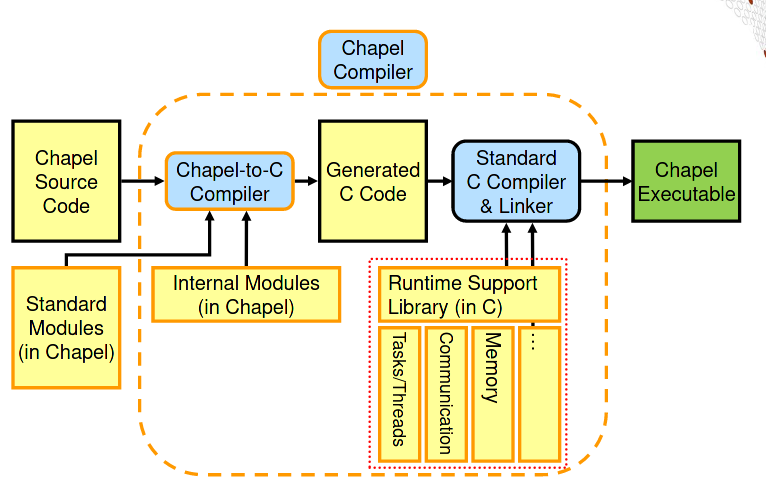
\includegraphics[width=0.65\textwidth]{Figures/chapel_arch.png}
        \label{fig:chapel_arch}
		\caption{Chapel Compilation and Runtime Architecture from \cite{chapel_rts_ppt}}
    \end{figure}
	\paragraph{Description}
	Like X10, Chapel attempts to solve the problem of providing a standard library for distributed computing through a new language instead of a framework that extends an existing language. Additionally, the design and development of Chapel, like that of X10, was led by an industry leader in high performance computing, Cray Inc. Chapel's original authors believed that the predominant mode of programming for HPC applications at the time, Fortran and/or C/C++ with MPI, was too low-level and demanding for typical programmers, comparing writing MPI programs in these languages to writing assembly code for single sequential processor machines \cite{chapel}.
	
	As mentioned in \ref{X10_desc}, there were many languages with the same goal as Chapel, so the authors attempted to differentiate themselves by aiming to outperform these languages while still offering the same abstractions to increase productivity. Chapel's four main goals at design time were to offer support for fine-grain parallelism, providde the infrastructure for locality-aware programming, allow for object-orientation, and allow for generic programming and type inference to simplify the type systems presented to users. Like X10, Chapel removes the notion of a thread from the language, eliminating many concurrent resource management issues from users. 

	One of the most important concepts in Chapel is that of a \textit{domain}. A Chapel domain is essentially a set of indices that supports parallel iterations \cite{chapel_2007}. This construct is used to support all of the data structures in Chapel, from sets to arrays to hash tables. Since the concept of domain is far more adaptive than the traditional array in other high-level programming languages, this results in a higher degree of flexibility when working with domains. For example, users can define domains with indexes that are floating points, strings, or references instead of just integers \cite{chapel_2007}. 

	Chapel's runtime system has a communication layer that supports inter-locale communicate, PUT/GET operations that work similarly to their HTTP equivalents, and remote fork operations which can be described as the distributed equivalent of the STL implementation of fork on a single system \cite{chapel_rts_ppt}. The runtime system's tasking layer is another abstraction of the concept of threads similarly to what exists in other libraries, offering synchronization and dependency support - the runtime system offers a distinct, "threading" layer to separate these tasks from the underlying thread programming.  The runtime system 
	\paragraph{Contributions}
	\begin{itemize}
		\item \textbf{Lightweight processors}. In \ref{introduction} and \ref{memory_distrib}, the prevalence of workloads that are dependent more on memory than processor performance is thoroughly discussed. The authors of Chapel noted this phenomenon as early as their first publication about the language in 2004, calling attention to the fact that large register sets/data caches are focused on a single thread, which can result in unncessarily large execution state and expensive context switching \cite{chapel}. In an attempt to remedy this, Cascade provides a distinct class of virtual processor, called a "lightweight" processor, that is optimized for programs which are either rich in short threads/synchronization or data intensive, and is implemented in the memory subsytem. While this project will likely never create a new virtual processor, this aspect of the Cascade architecture is intriguing, and using parts of this open implementation could be productive. 


		\item \textbf{Domain.} Chapel's concept of a domain, while implemented at the language level in their work, could be interesting as a generalization of an array within the context of a distributed C++ framework. Perhaps implementing an array with a more general indexing set as part of the library for this thesis project could lead to higher productivity and lower code reuse. 

	\end{itemize}

	\paragraph{Code sample}
	This code sample from \cite{chapel_github} demonstrates a distributed memory task parallel Hello World program in Chapel.
		
	\begin{lstlisting}[language=C++, caption=Hello World in Chapel, captionpos=b]
config const printLocaleName = true;


config const tasksPerLocale = 1;

coforall loc in Locales {

  on loc {

    coforall tid in 0\.\.#tasksPerLocale {

      var message = "Hello, world! (from ";

      if (tasksPerLocale > 1) then
        message += "task " + tid:string + " of " + tasksPerLocale:string + " on ";

      message += "locale " + here.id:string + " of " + numLocales:string;

      if printLocaleName then message += " named " + loc.name;

      message += ")";

      writeln(message);
    }
  }
}
	\end{lstlisting}

\subsection{memcached}
    \begin{figure}[h]
		\centering
		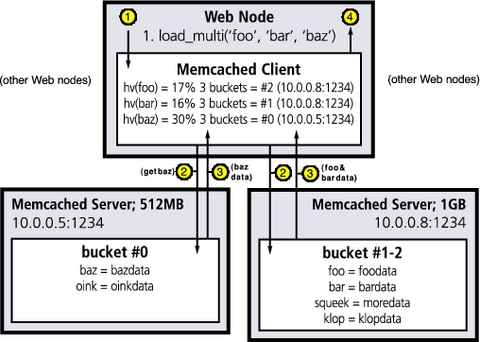
\includegraphics[width=0.65\textwidth]{Figures/memcached_arch.jpg}
		\label{fig:memcached_arch}
		\caption{Memcached Architecture from \cite{memcached_linux}}
    \end{figure}
	\paragraph{Description}
	Unlike all of the previous frameworks/languages previously explored, memcached is not a dialect/library of any other language, but rather an application, namely, a daemon, in and of itself. memcached was also originally created by Brad Fitzpatrick, a developer for LiveJournal who was looking to speed the retrieval of objects from memory on a webserver with in-memory caching \cite{lj_dev}. The application was first written in Perl, then was rewritten in C to eliminate inefficiencies inherent in Perl. 

	While memcached was originally only intended to serve pages and data from memory on LiveJournal, its use has expanded to the point where it is now a now a household name in industry. memcached is used on Twitter, Wikipedia, and many other high traffic sites to alleviate database load. Fitzpatrick recognized early on that CPU cycles were starting to get faster and faster, leading him to valuable to burn them over waiting for comparatively slower disks \cite{memcached_linux}. 

	Fitzpatrick was able to achieve his goal of using memory and CPU cycles over disk space whenever possible by creating a global hash table in which objects are stored as key-value pairs. memcached instances are run on every server with any memory over a cluster.  memcached utilizes a two-layer hash: the first layer decides to which memcached instance a request should be sent by hashing the key onto a list of virtual buckets (each a memcached instance), and then the memcached instance uses a typical hash table \cite{memcached_linux}. memcached can be run on servers with many different memory sizes, and is relatively machine  agnostic, meaning it does not depend upon the endian-ness or instruction set of a machine. 


	All memcached algorithms are $O(1)$, and it uses a slab allocator for memory allocation, generating slab classes of varying size. Memcached is also lockless, because objects are internally multiversioned and reference counted, meaning that no client can block another client's actions.  

	\paragraph{Contributions}
	\begin{itemize}
		\item \textbf{Redundant and lockless distributed memory.} While many approaches to distributed memory utilize at least some sort of locking mechanism, memcached does not. This allows for a far more usable product, and flattens the learning curve for users, as the only background knowledge needed is how to effectively utilize a dictionary. memcached also provides exceptional redundancy, as any node in a cluster can go down without affecting the performance of the overall service/website.  
		\item \textbf{Efficient load-balanced implementation of two-layer distributed hash table.} memcached may be a bit limited compared to the C/C++ libraries detailed earlier, but it does offer an excellent implementation of a distributed hash table. This could serve as a reference implementation for the maps/hash tables in this project. 
	\end{itemize}
